Giving the customer the possibility to participate in the development of a
product by providing him transparency regarding the overall progress and by 
implementing its feedback is one of the most important success factors.
Especially if the final results of the collaboration are not explicitly clear or
if the project is some kind of research work, it is of highest importance to
gather the customer�s feedback continuously. The gained feedback serves as an
input in adapting the product or even the whole process of development.

\begin{figure}
\centering
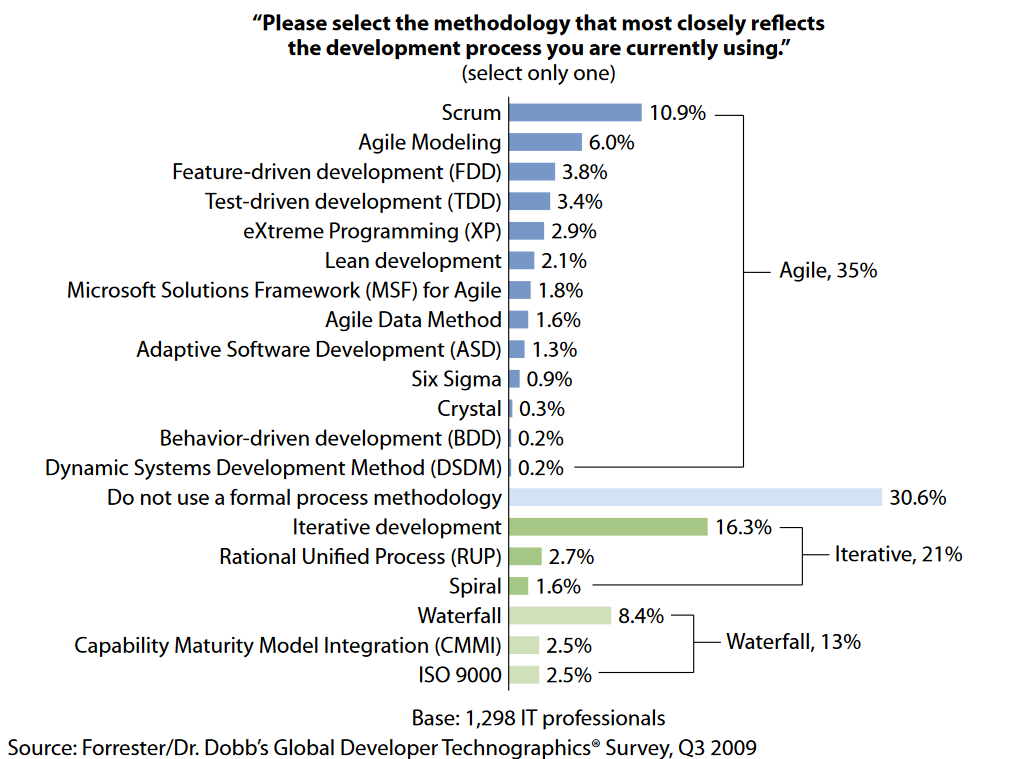
\includegraphics[width=0.75\textwidth]{res/applicationOfAgileMethods.PNG}
\caption{Adoption of agile Methods in Software Development (\cite{forrester})}
\label{fig:agileAdoption}
\end{figure}

Especially in the area of software development, the need for constant
interaction between a manufacturer and its customer is widely acknowledged. This
fact can be demonstrated by the adoption of agile methods (see figure
\ref{fig:agileAdoption}). These methods, like XP, Scrum and FDD, offer the
possibility of high transparency, short feedback-cycles and increased
flexibility regarding changes in the requirements or in the market -�
characteristics that proved themselves good and that are strongly wanted 
by the manufacturers adopting agile methods (see figure
\ref{fig:agileFeatures}).

\begin{figure}
\centering
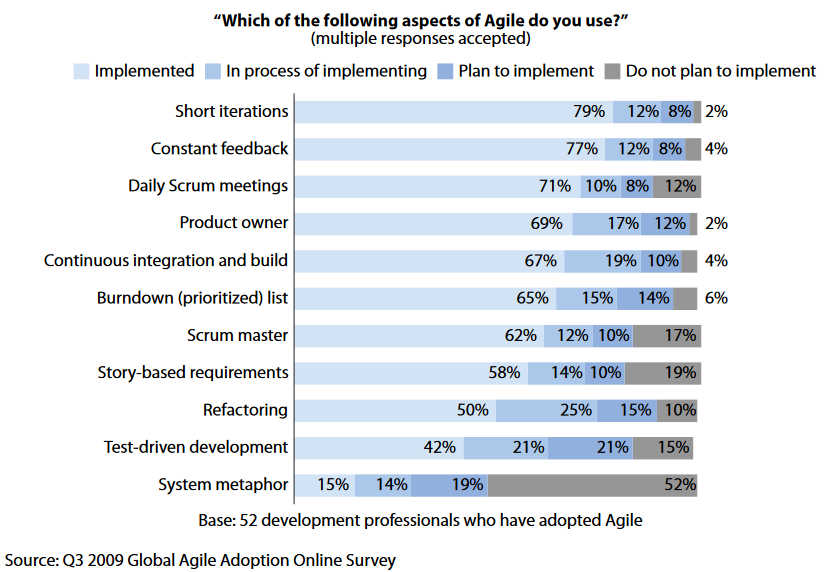
\includegraphics[width=0.75\textwidth]{res/aspectsOfAgile.PNG}
\caption{Adoption of agile Methods in Software Development (\cite{forrester})}
\label{fig:agileFeatures}
\end{figure}

\section{Determining the Modalities of Collaboration}
To embed a process that as well satisfies the customer as it provides the
manufacturer the possibility to get as much useful input and feedback as
possible, the modalities of collaboration are negotiated as a first step. The
salient points in this negotiation are:

\begin{itemize}
\item{Who is the customer's specialist contact person and how should the
communication with him/her take place?}
\item{Who is the customer's technical contact person and how should the
communication with him/her take place?}
\item{In which way will the customer contact our company if necessary=}
\item{What are the customers preferences regarding the reports on the project�s progress?}
\end{itemize}

While some of these points like the contact information of a certain person in
charge are only of informational kind, other points like the desired way of
communication are of high importance. Since there are certain preferences in our
company regarding the length of the iterations and the way how the communication
should take place, the CORE value of the customer�s answers in respect of our
company�s preferences is calculated.
